\chapter{Fahrkomfort und Einordnung in den Kontext Autonomes Fahren}\label{cha:Komfort}
In diesem Kapitel soll der Begriff ``Fahrkomfort'' in den Kontext des Autonomen Fahrens eingeordnet werden. Dazu wird zunächst die Bedeutung des Begriffs genauer betrachtet und die Verbindung zwischen Fahrkomfort und Sicherheitsempfinden dargelegt. Anschließend werden verschiedene Einflussfaktoren auf die Komfortwahrnehmung während des Fahrens thematisiert. Dabei wird das Phänomen der Kinetose genauer erklärt und speziell auf dessen Bedeutsamkeit für die Entwicklung autonomer Fahrzeuge eingegangen. Abschließend werden mithilfe von Literaturwerten Grenzwerte für die als relevant erarbeiteten Einflüsse untersucht. 

%\section{Begriffsdefinition Komfort}
%Während der Begriff ``Komfort'' im alltäglichen Sprachgebrauch eine sehr vielseitige Bedeutung hat und dabei sowohl zur Beschreibung positiver Empfindungen wie Wohlbehagen und Zufriedenheit, als auch in negierter Form zur Beschreibung negativer Gefühle wie Unwohlsein und Unzufriedenheit verwendet wird, wird bei der wissenschaftlichen Verwendung oftmals stärker differenziert. Es exisitieren verschiedene Modelle, die alle darauf abzielen, eine allgemeine Definition von Komfort zu liefern. Im Sinne der besseren Unterscheidbarkeit und damit einer genaueren Anwendung der entsprechenden Bedeutung, wird häufig zusätzlich der Begriff ``Diskomfort'' verwendet. In \cite{Zhang} wurden in einer Studie Faktoren für das Empfinden von Komfort und Diskomfort beim Sitzen identifiziert, wodurch sich die beiden Begriffe differenzierter verwenden lassen. Während Komfort durch Gefühle, die allgemein als positiv wahrgenommen werden, wie Entspanntheit, Ruhe und Zufriedenheit, klassifiziert wird, zeichnet sich Diskomfort vor allem durch negativ konnotierte Empfindungen, wie Müdigkeit und Rastlosigkeit, aber auch durch biometrische Faktoren, die spürbare Schmerzen verursachen, aus. Die Autoren leiten ein Modell her, in dem Komfort und Diskomfort zwei orthogonale Größen sind, die auch gleichzeitig erfahrbar sind. Während die Abwesenheit von Diskomfort nicht automatisch zur Zunahme von Komfort führt (dasselbe gilt auch anders herum), führt eine Zunahme von Diskomfort zwangsläufig zu einer Abnahme von Komfort. Wie Festner in \cite{Festner_diss} herausarbeitet, ist die Beseitigung von Diskomfort eine notwendige, jedoch nicht hinreichende Bedingung für das Empfinden von Komfort. Da jedoch unangenehme Situationen oftmals deutlicher explizit als solche wahrgenommen werden können, denn angenehme Situationen als angenehm, kann auch der erlebte Diskomfort als Kriterium für den fehlenden Komfort genutzt werden \cite{Festner}. 
%
%Ein weiteres Modell, welches breite Verwendung findet, ist die Komfortpyramide nach Krist \cite{Krist}. 
%\begin{figure}[h]
%	\centering
%	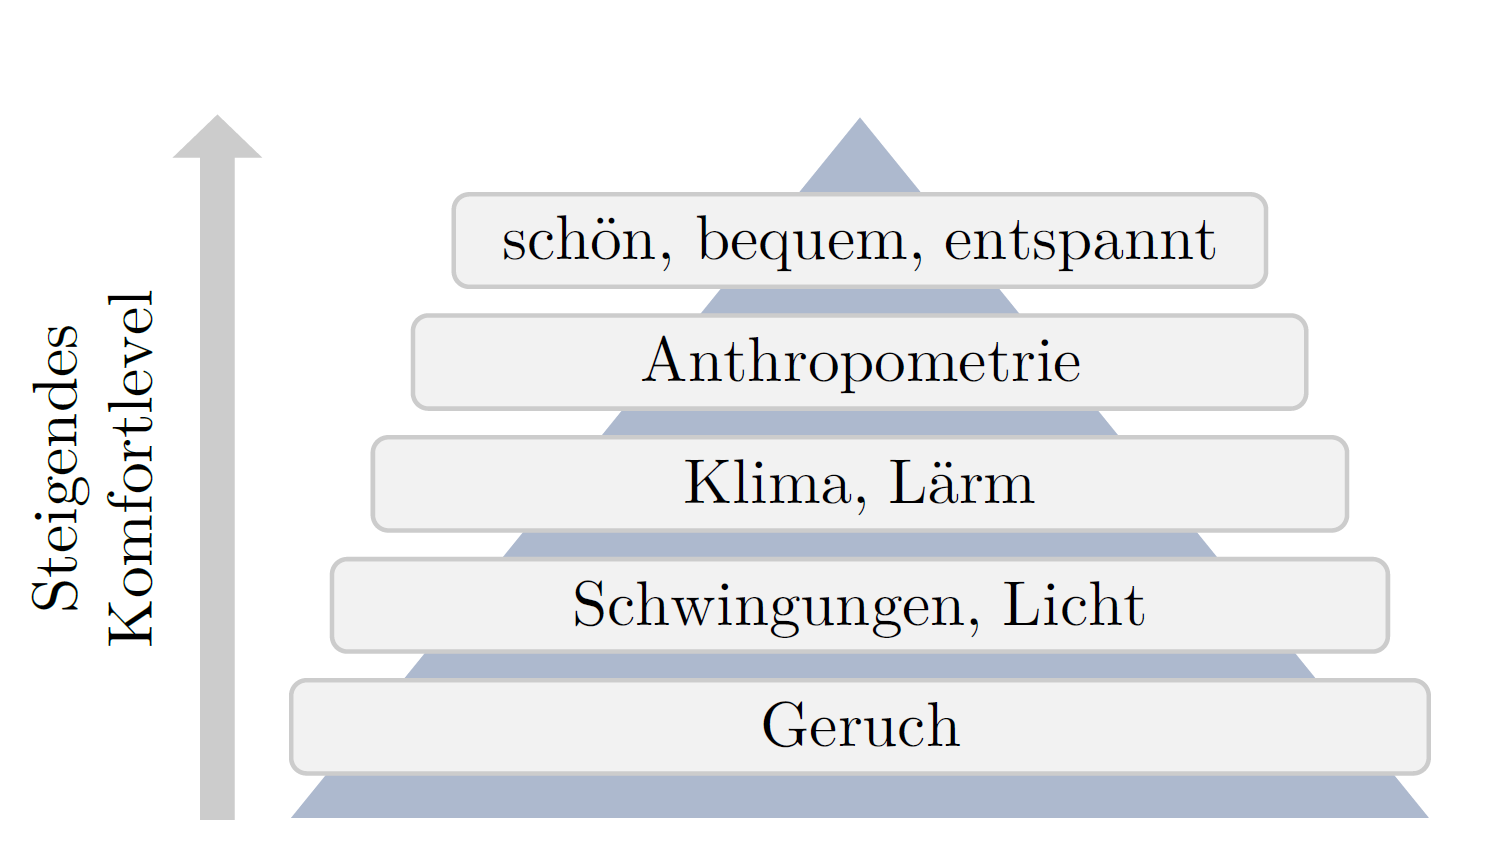
\includegraphics[scale=0.3]{./Bilder/komfortpyramide.png}
%	\label{fig:komfortpyramide}
%	\caption{Komfortpyramide aus \cite{Festner}, zitiert nach \cite{Krist}}
%\end{figure}
%
%In dieser Pyramide nimmt das Komfortlevel, ausgehend von sehr elementaren Faktoren wie Geruch und Lichteinflüssen, stetig zu. Um ein hohes Maß an Komfort zu erzielen, müssen notwendiger Weise zunächst die unteren, grundlegenden Bedingungen erfüllt sein. Zwar werden in diesem Modell Komfort und Diskomfort nicht so streng von einander getrennt, wie in \cite{Zhang}, allerdings ist die Bedingung, dass die Faktoren auf den unteren Ebenen zuerst erfüllt sein müssen damit auch auf den oberen Ebenen die Komfortbedingungen erfüllt werden können, vergleichbar mit der notwendigen Beseitigung von Diskomfort. Neben der qualitativen Beschreibung von Komfort, die alle Modelle gemein haben, unterscheiden sich die Ergebnisse, die unter Verwendung dieser Modelle erzielt werden, dennoch zum Teil stark, da die Komfortwahrnehmung sehr subjektiv ist und sich zwischen einzelnen Personen stark unterscheiden kann. Es lassen sich zwar einzelne Merkmale als komfortabel oder unkomfortabel klassifizieren, allerdings geht aus den Modellen nicht eindeutig hervor, wie stark die einzelnen Merkmale das persönliche Komfortempfinden beeinflussen. Zum Beispiel entwickelt jeder Mensch seine eigene Komfortpyramide, abhängig von ganz persönlichen Faktoren und Erfahrungen \cite{Krist}.
 
\section{Fahrkomfort im Kontext Autonomes Fahren}
Mit zunehmender Automatisierung von Fahraufgaben rückt auch der Fahrkomfort immer mehr in den Fokus. Es ist nicht davon auszugehen, dass FAS, die vom Fahrer als unkomfortabel empfunden werden, eine hohe Akzeptanz finden werden. \\
Damit sich überhaupt ein komfortables Gefühl während einer automatisierten Fahrt einstellen kann, muss beim Fahrer ein Gefühl von Sicherheit herrschen \cite{Festner.2019}. Nicht nur für unbeteiligte Dritte wie Fußgänger oder andere Autofahrer, sondern vor allem auch für den Fahrer spielt die Sicherheit bei autonomen Fahrzeugen daher eine zentrale Rolle. In \cite{Festner.2019} wird dabei der Unterschied zwischen subjektiver und objektiver Sicherheit dargelegt. Während das subjektive Sicherheitsempfinden lediglich wiedergibt, wie der Fahrer die Fahrt oder einzelne Situationen empfindet, lässt sich die objektive Sicherheit mithilfe von Größen wie reduzierten Unfallzahlen quantifizieren. Allerdings kann das subjektive Sicherheitsempfinden durchaus von der objektiven Sicherheit abweichen. Insbesondere bei FAS, die nach der SAE-Klassifizierung \cite{SAE klassifizierung} Stufe 3 oder höher zugeordnet werden, und bei denen damit das Fahrzeug nicht nur die Längs- und Querführung, sondern zusätzlich auch die Umfeldüberwachung übernimmt, kommt der in \cite{Elbanhawi.2015} als ``\textit{loss of controllability}'' eingeführte Paradigmenwechsel von Fahrer zum Passagier zum Tragen. Dadurch, dass der Fahrer mehr und mehr die Fahrzeugführung und Überwachung aller Funktionen an das Fahrzeug abgibt, stellt sich möglicherweise ein Gefühl von Kontrollverlust ein, weshalb nicht nur die objektive Sicherheit neuartiger Systeme eine große Rolle bei der Bewertung der Systeme spielt, sondern auch das subjektive Sicherheitsempfinden, welches eng an den wahrgenommenen Komfort geknüpft ist. \\
Neben dem Sicherheitsempfinden gibt es weitere wichtige Faktoren, die den Fahrkomfort beeinflussen. Großen Einfluss auf das Komfortempfinden hat dabei der Fahrstil. In verschiedenen Studien wurden unterschiedliche Fahrstile identifiziert und in verschiedene Klassen unterteilt \cite{Abendroth, B.; Bruder, R in Handbuch Fahrerassistenzsysteme, Bellem, Murphey}\cite{Abendroth.2009}\cite{Bellem.2016}\cite{Murphey.30.03.200902.04.2009}. So variiert zwar die Anzahl und genaue Bezeichnung der einzelnen Klassen zwischen den verschiedenen Studien, jedoch erstreckt sich das Spektrum immer von ``langsam'' oder ``komfortorientiert'' bis hin zu ``dynamisch/sportlich'' oder sogar ``aggressiv''. In \cite{Lange}\Cite{Lange.2014} konnte gezeigt werden, dass der Wunsch nach höherem Komfort mit dem Grad der Automatisierung steigt. Ein Grund für diesen Zusammenhang ist unter anderem, dass das Bedürfnis nach Feedback durch die Straße über das Fahrzeug an den Fahrer mit zunehmender Automatisierung geringer wird. Daher liegt für autonome Fahrzeuge im Alltagsgebrauch ein komfortorientierter Fahrstil nahe. 

Um beurteilen zu können, ob ein Fahrstil als komfortabel oder unkomfortabel wahrgenommen wird, muss zunächst geklärt werden, welche Merkmale dabei besonders großen Einfluss auf das Komfortempfinden haben. In \cite{scherer} wurden in einer Fahrsimulatorstudie die Merkmale Sicherheitsabstand zum Vorderfahrzeug, Bremsen, Geschwindigkeit, Beschleunigung, Spurhalten, Lenken und Blinkernutzung als die am häufigsten genannten Komfortkriterien identifiziert, wobei die drei ersten Merkmale von über der Hälfte der Teilnehmer als relevant erachtet wurden.\\
Neben den hier identifizierten Komfortmerkmalen lässt sich auch die Reisezeit als weiteres Kriterium angeben. Bereits in \cite{oborne}\cite{Oborne.1978} wurde dargelegt, dass Passagiere, die einer längeren Reisezeit ausgesetzt sind, ein höheres Maß an Komfort benötigen, als bei einer kürzeren Reisezeit. Jeder Passagier geht daher einen subjektiven Kompromiss zwischen der erwarteten Reisezeit und dem akzeptierten Niveau an Diskomfort ein. Aufgrund dessen hängen die vom Fahrer als komfortabel empfundenen biomechanischen Werte auch von der Reisezeit ab \cite{Festner.2019}.

Eine besondere Gewichtigkeit bei der Trajektorienplanung bezüglich des Fahrkomforts kommt dem Beschleunigungsverhalten zu. In \cite{Bellem}\cite{Bellem.2016} konnte in zwei Studien für verschiedene Fahrmanöver nachgewiesen werden, dass sich Merkmale wie Längs- und Querbeschleunigung sowie der Fahrzeugruck gut dazu eignen, einen komfortablen Fahrstil von anderen Fahrstilen abzugrenzen. Laut \cite{elbanhawi}\cite{Elbanhawi.2015} ist der häufigste Ansatz zur Optimierung der Fahrzeugbewegungen, die auf den Passagier wirkenden Kräfte und Rucke zu minimieren. Dass bei der Betrachtung des Beschleunigungsverhaltens jedoch nicht nur die absoluten Werte der Beschleunigung relevant sind, zeigen die Untersuchungen in \cite{gianna}\cite{Gianna.1996}. Hier konnte festgestellt werden, dass der Mensch bei lateralen Bewegungen insbesondere gegenüber Änderungen der Beschleunigung sehr sensitiv reagiert und diese besonders gut wahrnimmt. In \cite{dovgan} konnte ein Algorithmus entwickelt werden, der komfortable Fahrstrategien liefert, wobei als zusätzliches Komfortmerkmal der Ruck verwendet wurde. Dieser sollte dazu im Sinne des Fahrkomforts so gering wie möglich sein.

\subsection{Kinetose und ihre Bedeutung für das Autonome Fahren}\label{sec:kinetose}
Kinetose, oftmals auch als Reise- oder Bewegungskrankheit bezeichnet (\textit{engl.} Motion Sickness), beschreibt das Phänomen, dass man sich bei Reisen - vor allem im Auto, Flugzeug oder auf einem Schiff - plötzlich unwohl fühlt. Die Symptome reichen dabei von Blässe und leichter Übelkeit, über Schwindel und Kopfschmerzen, bis hin zum Erbrechen \cite{money}\cite{Money.1970}. Es existieren mehrere Theorien für die genauen Ursachen von Kinetose \cite{money}\cite{Money.1970}. Eine anerkannte und weit verbreitete Theorie für das Auftreten von Kinetose liegt dabei in einem visuell-vestibulären Sensorkonflikt \cite{motion sickness golding, motion sickness reason, motion sickness benson}\cite{Golding.2006}\Cite{Reason.1975}. Dadurch, dass Sensorinformationen über Beschleunigungen, die über das Gleichgewichtsorgan aufgenommen werden, nicht zu den Informationen passen, die über den visuellen Informationskanal geliefert werden, können die zuvor genannten Symptome auftreten. Dabei können prinzipiell alle Menschen mit einem funktionsfähigen Vestibularapparat gleichermaßen von Kinetose betroffen sein \cite{motion sickness lackner}\cite{Lackner.2014}. 

Neben dem Einfluss des Sensorkonflikts auf die Ausprägung von Kinetose, konnte in \cite{vogel motion sickness}\cite{Vogel.1982} außerdem gezeigt werden, dass starke, periodische Längsbeschleunigungen, die vor allem beim Bremsen auftreten, ebenfalls das Auftreten der Reisekrankheit begünstigen. 

Ein bekanntes Nebenphänomen der Reisekrankheit ist, dass sie überwiegend bei Beifahrern bzw. Passagieren, die nicht der Fahrer sind, auftreten \Cite{motion sickness reason}\Cite{Reason.1975}. In \cite{sivak motion sickness} und \cite{rolnick}\cite{Rolnick.1991} wurden mehrere Gründe für dieses Phänomen gefunden. Zum einen hat der Fahrer, als die Person, die das Fahrzeug steuert, die Kontrolle über die Fahrzeugbewegungen und damit auch die Richtung, in die sich die Fahrzeuginsassen bewegen. Dies ist bei den Beifahrern nicht der Fall und die fehlende Kontrolle führt zu einer größeren Anfälligkeit für die Reisekrankheit. Außerdem kann der Fahrer durch die ihm gegebene Kontrolle über das Fahrzeug Bewegungen besser antizipieren. In \cite{sivak motion sickness} wird außerdem der bereits erwähnte visuell-vestibuläre Sensorkonflikt als Grund angeführt, da Beifahrer die Möglichkeit haben sich fahrfremden Tätigkeiten zu widmen, wodurch der Sensorkonflikt verstärkt wird. Bei einer Umfrage zum Thema fahrfremder Tätigkeiten während der Fahrt mit einem vollständig selbst fahrenden Auto in \cite{sivak motion sickness} gab ein Großteil der über 3000 Befragten an, während der Fahrt andere Tätigkeiten als das Beobachten der Straße auszuüben. Gleichzeitig gaben zwischen 4 und 14 Prozent der Erwachsenen an, dass sie in vollständig selbst fahrenden Autos wahrscheinlich oft bis immer ein gewisses Maß an Kinetose verspüren würden. Die Ausprägung moderater bis schwerer Symptome tritt nach eigener Einschätzung bei zwischen 4 und 17 Prozent der Befragten auf. Diese Studie verdeutlicht die besondere Bedeutung, die der Reisekrankheit bei der Entwicklung autonomer Fahrzeuge zukommt. 

Kinetose besitzt aus zwei Gründen eine ausdrückliche Relevanz für die Komfortwahrnehmung beim Autonomen Fahren. Neben dem Einfluss von Beschleunigungen und Rucken, den diese bereits bei manueller, selbst gesteuerter Fahrt auf das Komfortempfinden haben, kommt nun noch dazu, dass auch das Risiko an Kinetose zu erkranken, maßgeblich vom Beschleunigungsverhalten abhängt. Des Weiteren tritt die Reisekrankheit überwiegend bei Beifahrern bzw. Passagieren auf, wodurch bei der Fahrt mit einem autonomen Fahrzeug erhöhtes Kinetoserisiko besteht, wenn sich der Fahrer nun anstelle der Fahraufgabe auf fahrfremde Tätigkeiten wie Zeitunglesen oder die Arbeit am Laptop oder Smartphone konzentrieren kann und dadurch immer mehr selbst zum Beifahrer wird. Dementsprechend besteht die Gefahr, dass Kinetose bei autonomen Fahrten vermehrt auftreten könnte, wodurch der Komfort drastisch reduziert wird. Es ist daher plausibel, dass den Ursachen von Kinetose bei der Entwicklung autonomer Fahrzeuge und der Planung der Fahrzeugbewegung durch entsprechende Maßnahmen entgegengewirkt werden sollte. 

Nachdem der Einfluss unterschiedlicher Faktoren auf den Fahrkomfort - insbesondere unter Berücksichtigung von Kinetose - analysiert wurde, lässt sich feststellen, dass im Beschleunigungsverhalten des Fahrzeugs - sowohl in longitudinaler als auch in lateraler Richtung - die wichtigsten Merkmale für die Komfortbetrachtung bei der Trajektorienplanung enthalten sind. Aus diesem Grund werden in dieser Arbeit neben der Reisezeit ausschließlich die Kriterien Längs- und Querbeschleunigung sowie Längs- und Querruck in verschiedenen Kombinationen als Gütekriterien und zur Beurteilung des Fahrkomforts verwendet. 

\section{Komfortgrenzen für Fahrzeugbeschleunigung und -ruck}
Für die Bewertung der Komfortkriterien hinsichtlich des Fahrkomforts ist es notwendig möglichst genaue Grenzwerte für diese anzugeben. Nachfolgend wird der Frage nachgegangen, inwiefern sich Grenzen der verwendeten Komfortkriterien Fahrzeugruck und -beschleunigung quantitativ bestimmen lassen. Die Grenzen werden anhand von Literaturwerten herausgearbeitet und getrennt nach Längs- und Querdynamik betrachtet.

\subsection{Grenzwerte für die Längsdynamik} 
Für die Begrenzung der Längsdynamik des Fahrzeugs soll zunächst ein Blick auf bestehende \acrshort{FAS} geworfen werden, die den Fahrer in der Längsführung des Fahrzeugs unterstützen. Die Systeme \acrshort{ACC} sowie \acrshort{FSRA} stellen dafür praxiserprobte Systeme dar, die als Orientierung verwendet werden können. Das \acrshort{FSRA} ist eine Systemerweiterung des Standard \acrshort{ACC}, dessen Funktionalität zusätzlich zum mittleren und hohen Geschwindigkeitbereich auch den niedrigen Geschwindigkeitsbereich ($v < \valunit{5}{m/s}$) abdeckt \cite{Winner handbuch FAS}\cite{Winner.2009}. In den ISO-Normen ISO 15622 \cite{iso15622} und ISO 22179 \cite{iso22179} werden die Funktionsgrenzen der beiden Systeme spezifiziert, welche auch in \cite{Winner handbuch FAS}\cite{Winner.2009} nachgelesen werden können. Geht man davon aus, dass der Betrieb autonomer Fahrzeuge im gesamten möglichen Geschwindigkeitsbereich vom Stillstand bis hin zu hohen Geschwindigkeiten, welche auf Autobahnen vorherrschen, möglich sein soll, so dienen die Funktionsgrenzen des \acrshort{FSRA} als erste Anhaltspunkte für autonome Fahrzeuge. \\
Beim \acrshort{FSRA} wird zwischen den einzelnen Geschwindigkeitsbereichen unterschieden. Bei hohen Geschwindigkeiten von $v>\valunit{20}{m/s}$ betragen die Grenzwerte für die maximal zur Verfügung stehende Beschleunigung bzw. Verzögerung $\amax = \valunit{2}{m/s^2}$ bzw. $\amin = \valunit{-3,5}{m/s^2}$ \cite{Winner handbuch FAS}. Im Bereich niedriger Geschwindigkeiten von $v < \valunit{5}{m/s}$ betragen die Funktionsgrenzen $\amax = \valunit{4}{m/s^2}$ bzw. $\amin = \valunit{-5}{m/s^2}$ \cite{Winner handbuch FAS}. Im dazwischen liegenden Geschwindigkeitsbereich dürfen die Höchstwerte für die Beschleunigung und Verzögerung abhängig von der gefahrenen Geschwindigkeit innerhalb der angegebenen Werte für hohe und niedrige Geschwindigkeiten liegen \cite{Winner handbuch FAS}\cite{Winner.2009}.\\
Der Grenzwert für den zulässigen Fahrzeugruck wird für hohe Geschwindigkeiten mit $\jmax = \valunit{2,5}{m/s^3}$ und für niedrige Geschwindigkeite mit $\jmax = \valunit{5}{m/s^3}$ angegeben, wobei dieser Wert sowohl für positive als auch negative Beschleunigungen gilt \cite{Winner handbuch FAS}\cite{Winner.2009}. Auch hier darf der maximale Fahrzeugruck bei mittleren Geschwindigkeiten je nach tatsächlicher Geschwindigkeit innerhalb dieser Grenzen liegen. \\
Somit sind erste Werte für Funktionsgrenzen in Längsrichtung abgesteckt, wobei beachtet werden muss, dass diese Werte als absolute, zulässige Maximalwerte zu verstehen sind, bei denen der Fahrkomfort noch nicht berücksichtigt wurde \cite{Festner.2019}. Es kann davon ausgegangen werden, dass die Komfortgrenzen für \acrshort{FAS} enger gefasst werden müssen als die reinen Funktionsgrenzen, weshalb die Grenzen unter Berücksichtigung des Komforts nun weiter eingeschränkt werden sollen.

In \cite{liu und wu} wird ein Modell zur Folgefahrt basierend auf dem Fahrer- bzw. Passagierkomfort vorgestellt. Als Schwellwert der Längsbeschleunigung für die Unterscheidung zwischen einer komfortablen und einer unkomfortablen Fahrt wird dabei der Wert $a_c = \valunit{2}{m/s^2}$ angegeben. In \cite{radke} wurde die mittlere Längsbeschleunigung eines ``undynamischen'' und damit als komfortorientiert empfundenen Fahrstils auf Landstraßen experimentell als \valunit{1}{m/s^2} ermittelt. 
\textbf{TODO: Längsverzögerung}

Für den Längsruck gilt laut \cite{Fun-to-Drive by Feedback} typischerweise für die Entwicklung vieler Anwendungen wie den Entwurf von Zugstrecken oder Personenaufzügen ein Grenzwert von $\jmax = \pm\valunit{2}{m/s^3}$ zur Wahrung des Passagierkomforts. Neben den absoluten Werten des Rucks konnte Hiroaki in einer Studie für das Railway Technical Research Institute in Japan zudem einen signifikanten Zusammenhang zwischen dem Ruck und der Beschleunigung bezüglich der Nutzerakzeptanz feststellen \cite{hiroaki}. Mit zunehmender Beschleunigung und größer werdendem Ruck sinkt die Akzeptanz eines Fahrmanövers.  


Die Ergebnisse in diesem Kapitel machen die Schwierigkeit bei der objektiven Bestimmung von Grenzwerten für den Fahrkomfort deutlich. Die Komfortwahrnehmung wird von einer Reihe unterschiedlicher Faktoren beeinflusst. Erst deren Gesamtwirken lässt sich je nach Situation und Fahrmanöver bezüglich des Fahrkomforts bewerten. Dazu kommt, dass das Komfortempfinden auch von subjektiven Eindrücken wie dem persönlichen Sicherheitsempfinden oder eigenen Fahrgewohnheiten geprägt wird. Allgemeingültige Werte, die als ``harte'' Komfortgrenzen verstanden werden können, können deshalb ohne zusätzliche Annahmen und Vereinfachungen nicht getroffen werden. Die in diesem Kapitel erarbeiten Grenzwerte für die komfortrelevanten Größen Fahrzeugruck und -beschleunigung in longitudinaler und lateraler Richtung dienen daher eher als Orientierung für die qualitative Bewertung des Fahrkomforts.
